\documentclass[tikz,border=7pt]{standalone}
\usetikzlibrary{calc}
\begin{document}
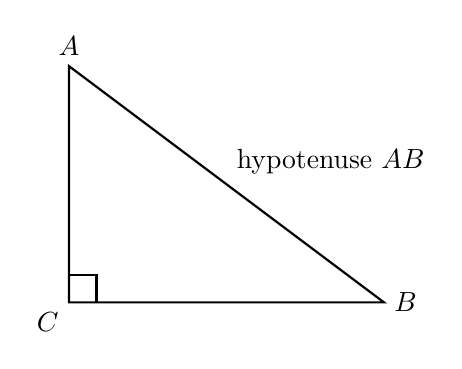
\begin{tikzpicture}[line width=.8pt]
\coordinate (C) at (0,0); \coordinate (A) at (0,3); \coordinate (B) at (4,0);
\draw (A)--(B)--(C)--cycle;
\draw (0,.35)--(.35,.35)--(.35,0);
\node[above] at (A) {$A$}; \node[right] at (B) {$B$}; \node[below left] at (C) {$C$};
\node[above right] at ($(A)!.5!(B)$) {hypotenuse $AB$};
\end{tikzpicture}
\end{document}
